\FloatBarrier
\section{Breaking with an eddy viscosity, and the longshore current}
\label{sec:brk}

The hydrostatic front approximation puts the breaking point in the right
place, but the bores of the surf zone lose too little energy
(Sections~\ref{sec:breaking} and \ref{sec:wd-tk}): only the one or two
columns at the front are flagged, and the non-hydrostatic pressure behind
them keeps the bores steep. This section adds the two ingredients of the
eddy-viscosity breaking model of \citet{kennedy2000} to the HFA
(Section~\ref{sec:hfa}): a persistence threshold that falls with the age of
the breaking event, so that the breaking region grows over the face of a
mature bore, and a breaking eddy viscosity in the breaking columns. It also
adds the kinematic onset criterion. The combinations are tested on the two
spilling-breaker cases, with the undertow of \citet{ting1994}, and the
default is then used for the last test of \citet{ma2012}, the longshore
current on a plane beach, which needs breaking, wetting and drying, bottom
friction and lateral mixing in 3D.

\subsection{Spilling breakers}
\label{sec:brk-spill}

The beach of \citet{ting1994} is run as in Section~\ref{sec:wd-tk} (10
layers, $\Delta x = 2.5$ cm, $\Delta t = 5$ ms, 60 s), now with the time
averages of the last 10 periods for the undertow. The variants differ only in
the breaking model (Table~\ref{tab:brk-tk}, Figs.~\ref{fig:brk-tk} and
\ref{fig:brk-undertow}):
\begin{itemize}[nosep]
  \item HFA: $\alpha = 0.6$, $\beta = 0.3$ \citep{smit2013}, as before;
  \item HFA with the breaking age: $\beta$ falls to $\beta_F = 0.15$ over
        $T^* = 5\sqrt{D/g}$;
  \item HFA and eddy viscosity (\code{hybrid}, the new default): the same
        threshold, $\delta_b = 1.2$, horizontal mixing;
  \item the same with vertical mixing as well (\code{verticalMixing yes});
  \item eddy viscosity alone, with vertical mixing (the non-hydrostatic
        pressure kept in the breaking columns);
  \item the default with the kinematic onset, $B_k = 0.85$.
\end{itemize}

\begin{table}[!htbp]
\centering
\caption{Spilling breakers of \citet{ting1994}: wave height $H$ and mean
water level $\bar\eta$ (cm), and the strongest undertow below the trough
level relative to the measured one (mean over the stations at
$x > 6.5$ m). Kinematic onset: $B_k = 0.85$; NHWAVE: $k$--$\epsilon$ with
20 layers.}
\label{tab:brk-tk}
\small
\setlength{\tabcolsep}{4pt}
\begin{tabular}{lcccccc}
\toprule
 & largest $H$ & $H$ & $H$ & mean error & $\bar\eta$ & undertow \\
 & (at $x$) & 8 m & 11 m & of $H$, $x > 7$ m & 11 m & \\
\midrule
lab & 16.5, 6.0 m & 9.3 & 3.9 & & 1.4 & 1 \\
HFA & 17.3, 6.4 m & 15.3 & 10.0 & $+6.1$ & 0.5 & 1.03 \\
HFA, breaking age & 17.2, 6.5 m & 14.9 & 9.8 & $+5.8$ & 0.6 & 0.91 \\
HFA + eddy viscosity & 17.6, 6.2 m & 12.9 & 6.6 & $+3.5$ & 0.8 & 1.32 \\
\quad with vertical mixing & 17.7, 6.3 m & 13.4 & 8.1 & $+4.4$ & 1.1 & 0.65 \\
eddy viscosity alone & 18.0, 6.5 m & 13.2 & 8.0 & $+4.1$ & 1.2 & 0.62 \\
kinematic onset & 21.1, 7.1 m & 13.0 & 5.3 & $+3.1$ & 0.9 & 1.38 \\
NHWAVE & 18.0, 6.9 m & 16.1 & 6.4 & $+4.8$ & 0.0 & 1.63 \\
\bottomrule
\end{tabular}
\end{table}

\begin{figure}[!htbp]
\centering
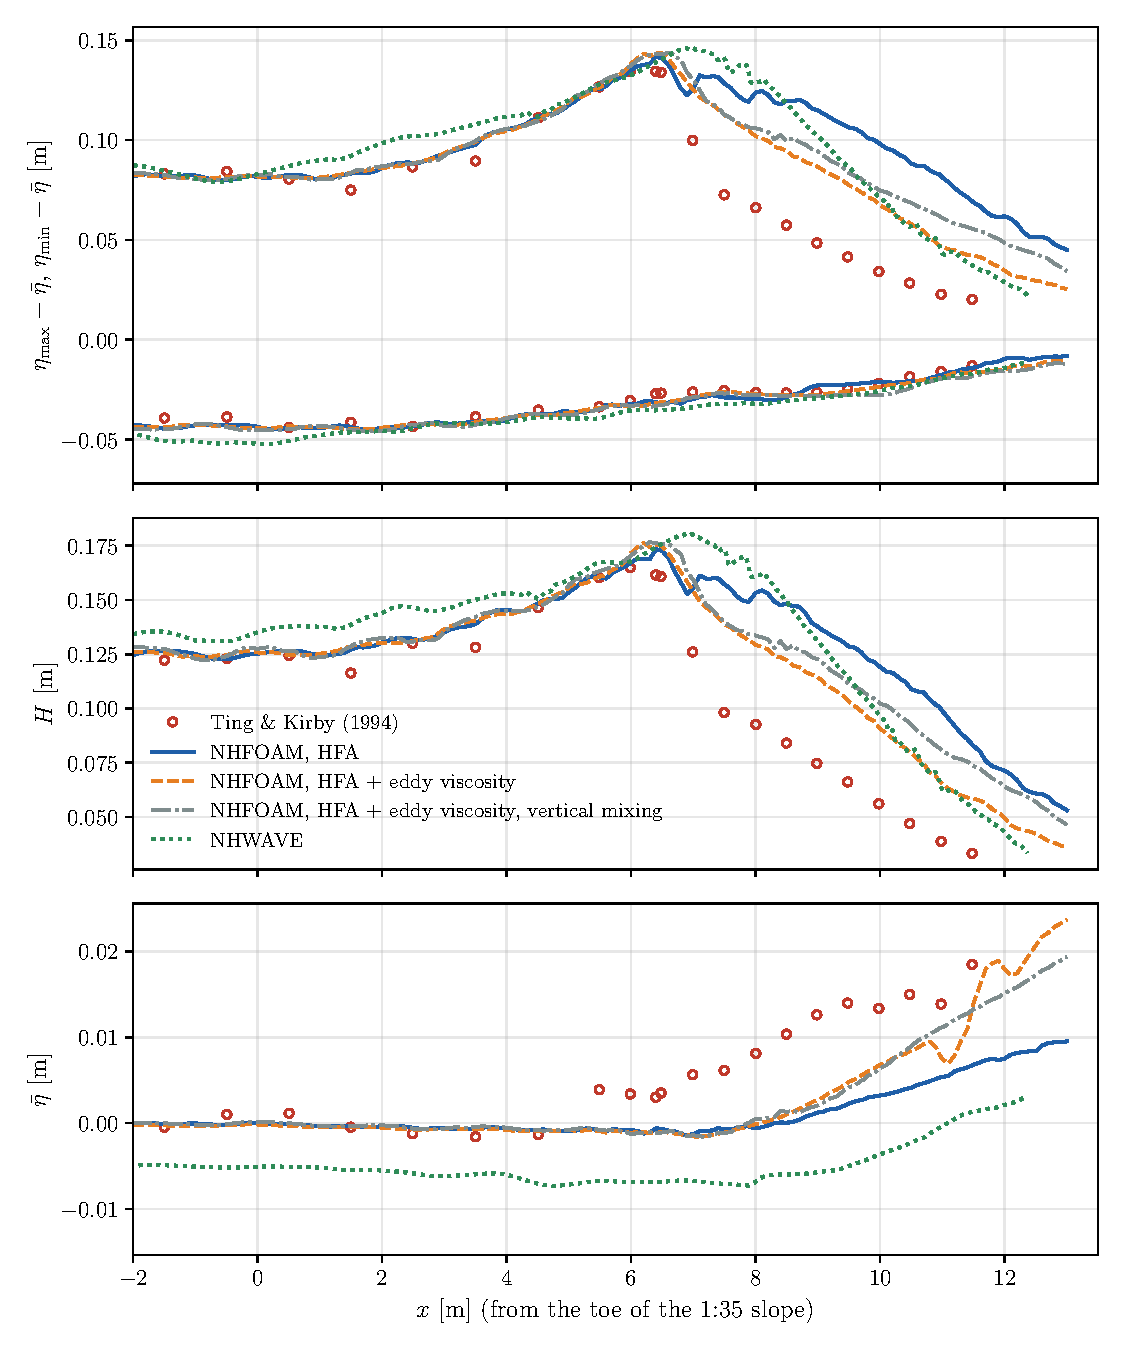
\includegraphics[width=0.9\textwidth]{tk_breaking.pdf}
\caption{Spilling breakers \citep{ting1994} with the breaking models: crest
and trough relative to the mean level, wave height and mean water level.}
\label{fig:brk-tk}
\end{figure}

\begin{figure}[!htbp]
\centering
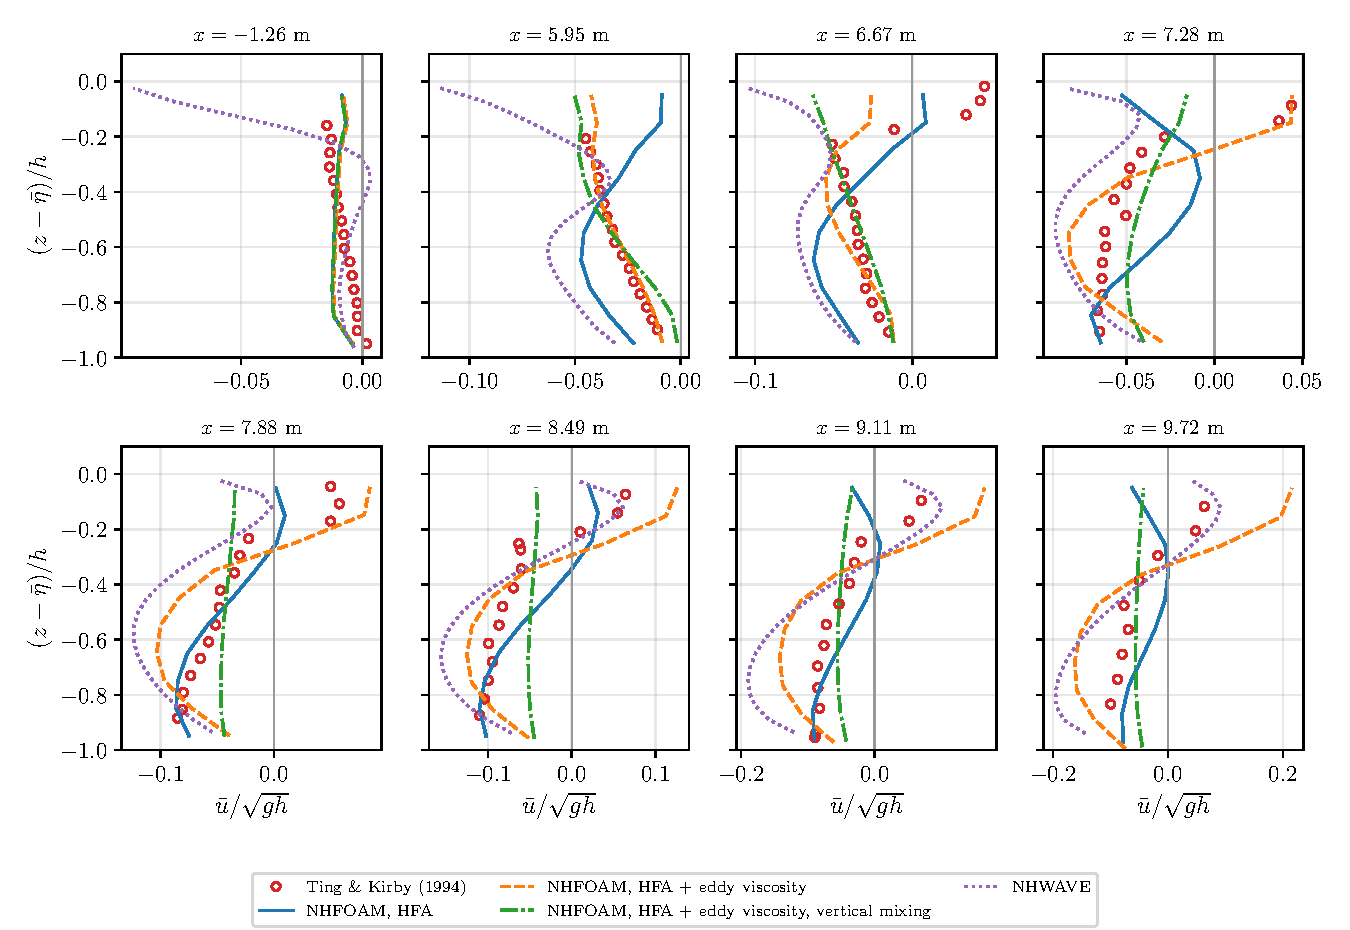
\includegraphics[width=\textwidth]{tk_undertow.pdf}
\caption{Spilling breakers \citep{ting1994}: time-mean horizontal velocity.
The models are averaged at fixed $\sigma$ and plotted at the mean height of
each level; above the trough level ($(z-\bar\eta)/h \gtrsim -0.25$) this is
not the Eulerian mean of the measurements.}
\label{fig:brk-undertow}
\end{figure}

The eddy viscosity makes the difference. With horizontal mixing (the
default), the mean error of the wave height in the surf zone falls from
$+6.1$ cm with the HFA alone to $+3.5$ cm, below NHWAVE's $+4.8$ cm with
$k$--$\epsilon$ and 20 layers, and the mean level near the shoreline rises
towards the measured one (0.8 cm at $x = 11$ m, lab 1.4 cm, HFA 0.5 cm).
The breaking age alone, which lets the hydrostatic region grow over the
face of the bore, changes little ($+5.8$ cm). The eddy viscosity without the HFA ($+4.1$ cm, with vertical mixing)
is close to the hybrid with vertical mixing ($+4.4$ cm): once $\nu_b$ acts,
the hydrostatic front adds little, and the dissipation comes from the eddy
viscosity. Vertical mixing through the layer faces dissipates less and
makes the undertow nearly uniform over the depth, at about 0.65 of the
measured strongest offshore velocity. Without it the profiles keep the
measured shape, onshore near the crests and offshore below, with the
strongest undertow 30\% too large (NHWAVE: 60\%); the HFA alone gives the
right strength but a weaker shear (Fig.~\ref{fig:brk-undertow}). Horizontal
mixing is therefore the default. The kinematic onset with $B_k = 0.85$
breaks 1.1 m late, at a height of 21 cm: with $\sqrt{gD}$ for the crest
speed, the surface velocity reaches $0.85\sqrt{gD}$ only when the wave is
about to overturn. Its smaller mean error inside the surf zone ($+3.1$ cm)
hides the 8 cm overshoot at the breaking point; the criterion needs a better
estimate of the crest speed, for instance from tracking the crests.

All variants keep the same main error, in the transition just after the
breaking point. Between $x = 6.4$ and 8 m the measured height drops from 16.2
to 9.3 cm, that of the models with the eddy viscosity by 4.2--4.6 cm only
(HFA alone 2.0 cm, NHWAVE 1.3 cm); further inshore their decay rates are
close to the measured one (Fig.~\ref{fig:brk-tk}). The eddy
viscosity starts at the onset, but the breaking region covers the face of
the bore only as the breaking event ages ($T^* \approx 0.75$ s at the
breaking point), while the measured breakers lose their height at once. In
a first version, columns joined a breaker at the lower threshold of an old
breaker. In this 2DV case that cut the error of the run with vertical mixing
from $+4.4$ to $+3.5$ cm, but on the beach of Section~\ref{sec:brk-ls} the
breaking region then crept along the crests of the oblique waves into deep
water, where it flagged waves 5 m from the shoreline; columns now join at
$\beta\sqrt{gD}$, the threshold of a new breaker.

On the spilling breakers of \citet{hansen1979} (Section~\ref{sec:breaking};
the same set-up, with the shelf and the velocity-only sponge), the default
nearly halves the error of the wave height in the surf zone, from an rms of 2.98 to
1.54 cm for $x > 8.3$ m ($-19\%$ to $+49\%$ of the measured heights instead of
$+3\%$ to $+99\%$), and that of the mean water level, from 4.6 to 2.2 mm,
with the same error before breaking (0.56 cm). It breaks 0.6 m early, with
the largest height 0.3 cm below the measured one (Fig.~\ref{fig:brk-hs}).

\begin{figure}[!htbp]
\centering
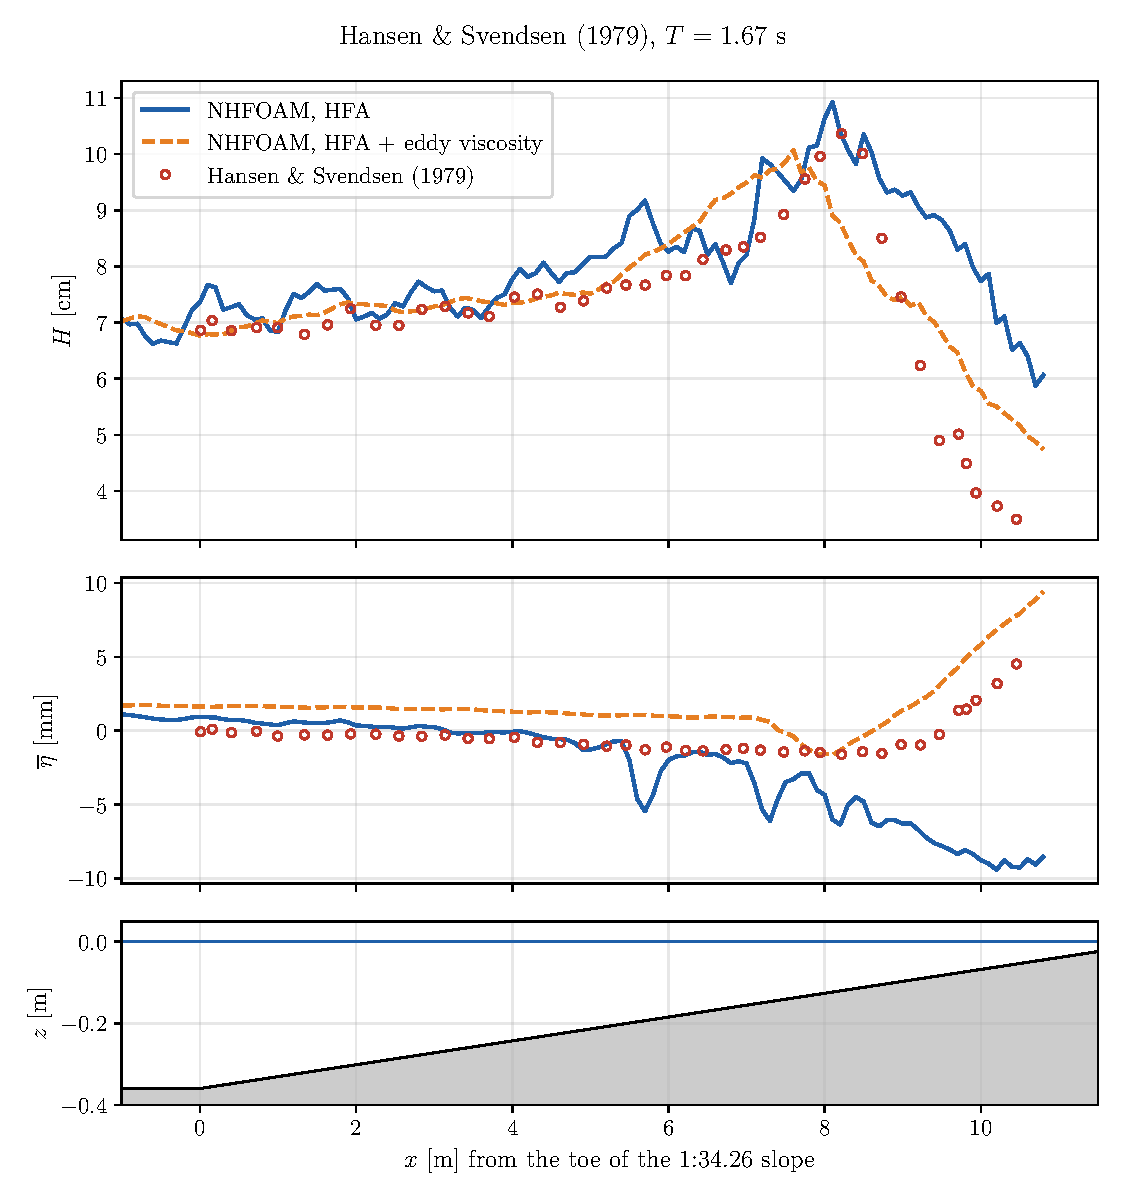
\includegraphics[width=0.85\textwidth]{hs_breaking.pdf}
\caption{Spilling breakers of \citet{hansen1979}: wave height and mean water
level with the HFA and with the default breaking model (HFA and eddy
viscosity).}
\label{fig:brk-hs}
\end{figure}

\subsection{Longshore current on a plane beach}
\label{sec:brk-ls}

\citet{visser1991}, experiment 4, is test 4.7 of \citet{ma2012}: regular
waves, $H = 7.8$ cm and $T = 1.02$ s, arrive at $15.4^\circ$ from the shore
normal over $h = 0.35$ m and break on a smooth concrete beach of slope 1:20,
driving a longshore current. The measurements used here are those tabulated
by \citet{kraus1991}: the wave height, the mean water level and the
depth-averaged longshore current, $(V_s + 2V_m + V_b)/4$ from dye at the
surface, at mid-depth and near the bottom. Visser reports the breaker line
2.51 m and the plunge line 1.92 m from the still-water shoreline, and a
largest current of 0.404 m/s.

Both models are periodic alongshore over one alongshore wavelength,
$L_y = 2\pi/(k\sin\theta)$, and use five uniform layers, log-law friction
with $k_s = 0.8$ mm (the value \citet{ma2012} found by tuning), the
Smagorinsky model with $\Delta = (\Delta x\,\Delta y\,\Delta\sigma D)^{1/3}$
and $C_s = 0.168$, and a 5 mm film; both run for 100 s, and the statistics
use the last five periods (Table~\ref{tab:brk-ls-setup}). \citet{ma2012} ran
NHWAVE on $280\times128$ cells; here both models have the same, coarser
grid, $\Delta x = 4$ cm and 32 (NHWAVE, a power of two for its periodic
boundaries) or 40 (\NHFOAM) cells alongshore, which is the affordable size
on the two cores used for this report. Because the crests are oblique, the
spacing along the wave direction is $\Delta y\sin\theta = 3.7$--4.6 cm, close
to $\Delta x$. \NHFOAM\ runs with the default breaking model of the previous
section, with HFA alone, and with the vertical mixing of the eddy viscosity.

\begin{table}[!htbp]
\centering
\caption{Longshore current: set-up of the two models.}
\label{tab:brk-ls-setup}
\small
\begin{tabular}{lp{5.8cm}p{5.2cm}}
\toprule
 & \NHFOAM & NHWAVE \\
\midrule
domain & 2 m flat (1.5 m wave zone), slope, 0.6 m land & 0.6 m flat, slope, 0.8 m land \\
cells & $240 \times 40 \times 5$, $L_y = 5.600$ m & $210 \times 32 \times 5$, $L_y = 5.533$ m \\
waves & stream function ($N = 24$), relaxation zone & linear, left boundary \\
time step & 10.2 ms (BDF2) & CFL 0.5 (about 9 ms) \\
breaking & HFA + eddy viscosity (or HFA) & shock capturing and Smagorinsky \\
turbulence & Smagorinsky (OpenFOAM LES library) & Smagorinsky (\code{IVTURB = 20}) \\
friction & log law, $k_s = 0.8$ mm & log law, \code{Zob} = 0.8 mm \\
\bottomrule
\end{tabular}
\end{table}

\begin{figure}[!htbp]
\centering
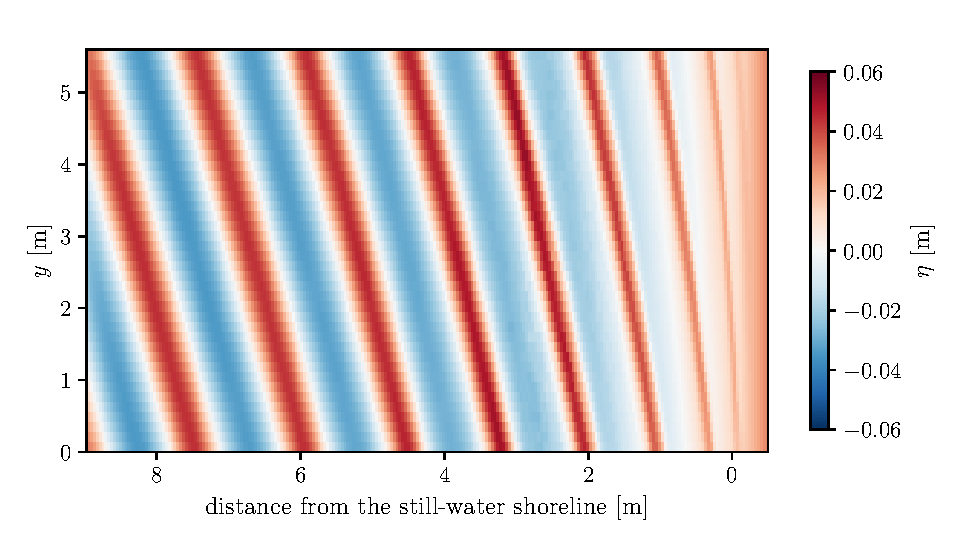
\includegraphics[width=0.8\textwidth]{longshore_snapshot.pdf}
\caption{Longshore current \citep{visser1991}: surface elevation of \NHFOAM\
at $t = 100$ s (default breaking model). The wave zone ends 7.5 m from the
shoreline.}
\label{fig:brk-ls-snap}
\end{figure}

\begin{figure}[!htbp]
\centering
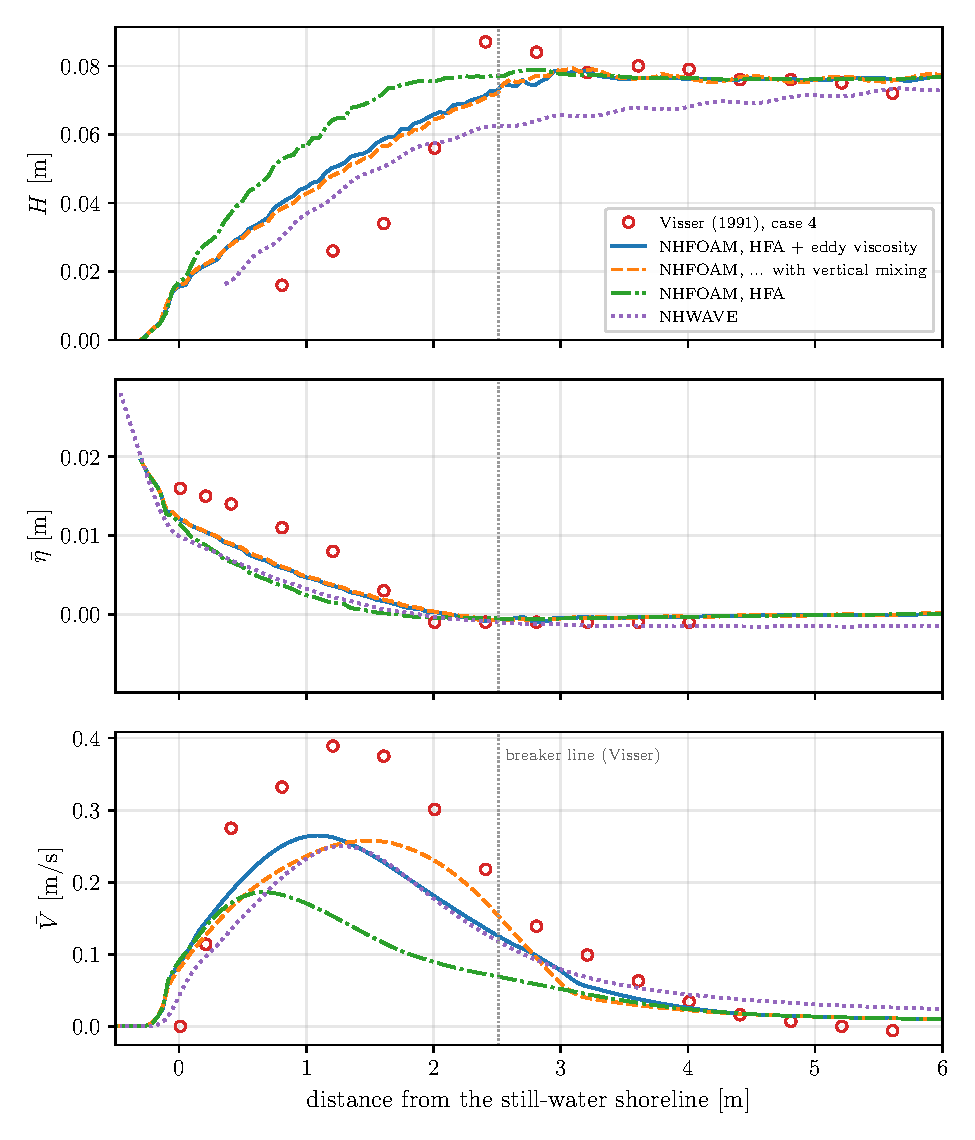
\includegraphics[width=0.85\textwidth]{longshore.pdf}
\caption{Longshore current \citep{visser1991}, case 4: wave height, mean
water level and depth-averaged longshore current, averaged over the last five
periods of 100 s and alongshore. NHWAVE's wave height needs zero crossings
and is not defined in the swash.}
\label{fig:brk-ls}
\end{figure}

\begin{table}[!htbp]
\centering
\caption{Longshore current: wave height at the measured breaking point
(2.41 m from the shoreline) and inside the surf zone (1.21 m), mean water
level at the shoreline, the largest longshore current and its distance from
the shoreline, and rms errors at the measuring stations. \code{hybrid}: HFA
and eddy viscosity (the default).}
\label{tab:brk-ls}
\small
\setlength{\tabcolsep}{4pt}
\begin{tabular}{lcccccc}
\toprule
 & $H$, 2.41 m & $H$, 1.21 m & $\bar\eta$, shore- & largest $\bar V$ & rms error & rms error \\
 & (cm) & (cm) & line (cm) & (m/s), at (m) & $H$ (cm) & $\bar V$ (m/s) \\
\midrule
lab & 8.7 & 2.6 & 1.6 & 0.39, 1.21 & & \\
\NHFOAM, \code{hybrid} & 7.1 & 5.0 & 1.2 & 0.265, 1.08 & 1.3 & 0.074 \\
\quad with vertical mixing & 7.1 & 4.8 & 1.2 & 0.258, 1.48 & 1.2 & 0.071 \\
\NHFOAM, HFA & 7.7 & 6.4 & 1.1 & 0.186, 0.68 & 1.9 & 0.123 \\
NHWAVE & 6.2 & 4.2 & 0.7 & 0.250, 1.26 & 1.3 & 0.082 \\
\bottomrule
\end{tabular}
\end{table}

The crests turn towards the shore over the slope (Fig.~\ref{fig:brk-ls-snap}).
In \NHFOAM\ the waves start breaking about 2.85 m from the shoreline, 0.35 m
seaward of Visser's breaker line, at 7.9 cm instead of the measured 8.7 cm,
and inside the surf zone their heights stay above the measured ones, as on
the two 2DV beaches (Fig.~\ref{fig:brk-ls}, Table~\ref{tab:brk-ls}). The
set-up at the shoreline is 1.2 cm (lab 1.6 cm). NHWAVE's waves lose height
on this grid before they break, from 7.9 cm at the wavemaker to 6.2 cm at
the measured breaking point.

Both models put the longshore current in about the right place but give two
thirds of its strength: 0.265 m/s at 1.08 m from the shoreline (\NHFOAM) and
0.250 m/s at 1.26 m (NHWAVE), against 0.39 m/s at 1.21 m. With the HFA alone
the waves keep more of their height inside the surf zone, and the current is
weaker, 0.19 m/s, with its peak at 0.68 m, close to the shoreline: the
behaviour \citet{ma2012} found when they switched off the turbulent
diffusion. The breaking eddy viscosity mixes the current across the surf
zone as well as dissipating the waves; with vertical mixing as well the peak
moves to 1.48 m. The current is uniform alongshore (over the columns at one
cross-shore position, the standard deviation of the mean depth-averaged
current is below 0.003 m/s), the mean
cross-shore velocity is an undertow of up to 4.6 cm/s, and the current still
builds up slowly: its peak grew by 2\% between 90 and 100 s.

\citet{ma2012} report the current well predicted by NHWAVE on their finer grid
($\Delta x = 3$ cm, $\Delta y$ three to four times smaller than here), so the
resolution of this grid is the likely main cause of the deficit both models
share; in \NHFOAM\ the slow decay of the heights after breaking also spreads
the forcing over a wider surf zone. On this grid each model took about 70 min
on one core (\NHFOAM: 48\,000 cells and 9800 steps; NHWAVE: 33\,600 cells);
the finer grid would take several hours on the two cores used here and is
left for a later run.
